
\documentclass[11pt, titlepage, oneside, a4paper]{article}
\usepackage{array}
\usepackage[T1]{fontenc}
\usepackage[utf8]{inputenc}
\usepackage[english]{babel}
\usepackage{amssymb, graphicx, fancyhdr}
\addtolength{\textheight}{20mm}
\addtolength{\voffset}{-5mm}
\renewcommand{\sectionmark}[1]{\markleft{#1}}

% \Section ger mindre spillutrymme, använd dem om du vill
\newcommand{\Section}[1]{\section{#1}\vspace{-8pt}}
\newcommand{\Subsection}[1]{\vspace{-4pt}\subsection{#1}\vspace{-8pt}}
\newcommand{\Subsubsection}[1]{\vspace{-4pt}\subsubsection{#1}\vspace{-8pt}}
	
% appendices, \appitem och \appsubitem är för bilagor
\newcounter{appendixpage}

\newenvironment{appendices}{
	\setcounter{appendixpage}{\arabic{page}}
	\stepcounter{appendixpage}
}

\newcommand{\appitem}[2]{
	\stepcounter{section}
	\addtocontents{toc}{\protect\contentsline{section}{\numberline{\Alph{section}}#1}{\arabic{appendixpage}}}
	\addtocounter{appendixpage}{#2}
}

\newcommand{\appsubitem}[2]{
	\stepcounter{subsection}
	\addtocontents{toc}{\protect\contentsline{subsection}{\numberline{\Alph{section}.\arabic{subsection}}#1}{\arabic{appendixpage}}}
	\addtocounter{appendixpage}{#2}
}

% Ändra de rader som behöver ändras
\def\inst{Datavetenskap}
\def\typeofdoc{Laborationsrapport}
\def\course{Systemnära Programmering 7,5 hp}
\def\pretitle{Laboration 5}
\def\title{mfind\_p}
\def\name{Christer Jakobsson}
\def\username{dv12cjn}
\def\email{\username{}@cs.umu.se}
\def\path{edu/sysprog/lab5}
\def\graders{Mikael Rännar, Adam Dahlgren Lindström, Niklas Fries, Oskar Ottander}


% Om du vill referera till katalogen där dina filer ligger kan du 
% använda \fullpath som kommer att vara "~username/edu..." o.s.v.
\def\fullpath{\raisebox{1pt}{$\scriptstyle \sim$}\username/\path}


% Här brjar själva dokumentet
\begin{document}

	% Skapar framsidan (om den inte duger: gör helt enkelt en egen)
	\begin{titlepage}
		\thispagestyle{empty}
		\begin{large}
			\begin{tabular}{@{}p{\textwidth}@{}}
				\textbf{UMEÅ UNIVERSITET \hfill \today} \\
				\textbf{Institutionen för \inst} \\
				\textbf{\typeofdoc} \\
			\end{tabular}
		\end{large}
		\vspace{10mm}
		\begin{center}
			\LARGE{\pretitle} \\
			\huge{\textbf{\course}}\\
			\vspace{10mm}
			\LARGE{\title} \\
			\vspace{15mm}
			\begin{large}
				\begin{tabular}{ll}
					\textbf{Namn} & \name \\
					\textbf{E-mail} & \texttt{\email} \\
					\textbf{Sökväg} & \texttt{\fullpath} \\
				\end{tabular}
			\end{large}
			\vfill
			\large{\textbf{Handledare}}\\
			\mbox{\large{\graders}}
		\end{center}
	\end{titlepage}


	% Fixar sidfot
	\lfoot{\footnotesize{\name, \email}}
	\rfoot{\footnotesize{\today}}
	\lhead{\sc\footnotesize\title}
	\rhead{\nouppercase{\sc\footnotesize\leftmark}}
	\pagestyle{fancy}
	\renewcommand{\headrulewidth}{0.2pt}
	\renewcommand{\footrulewidth}{0.2pt}

	% Skapar innehållsförteckning.
	% Tänk på att köra latex 2ggr för att uppdatera allt
	\pagenumbering{roman}
	\tableofcontents
	
	% och lägger in en sidbrytning
	\newpage

	\pagenumbering{arabic}

	% I Sverige har vi normalt inget indrag vid nytt stycke
	\setlength{\parindent}{0pt}
	% men däremot lite mellanrum
	\setlength{\parskip}{10pt}

	% Lägger in rubrik (finns \section, men då får man mycket spillutrymme)
	\Section{Problemspecifikation}
		% \emph innebär emphasize, d.v.s. betona eller framhåll -> kursiv stil
		\emph{Denna laborationsuppgift har handlat om att ta ett existerande program som skrivits under kursen och göra en trådad variant av det.}

		% lägg in en underrubrik (\subsection -> spillutrymme)
		\Subsection{Problemsammanfattning}
		Denna laboration har gått ut på att ta det fungerande programmet \emph{mfind} som skapades i laboration 3 och sedan göra så att istället för att använda en tråd för arbetet så används flera trådar.
		\emph{mfind} är ett program som söker efter en fil i systemet, liknande linux inbyggda \emph{find}. Det tar minst två argument. Vart sökningen skall börja och vilken fil som söks, det kan även 
		ta ett argument \\ \emph{-t filtyp} där filtyp kan vara f för vanlig fil, d för en katalog och l för en länk. Om detta argument specifierats så ska programmet bara söka efter den sortens fil.
		
		Detta är grunden i det program som jag har modifierat för att göra sökningen med flera trådar, vilket var vad denna uppgift gått ut på.
		
		\Subsection{Originalspecifikation}
			Specifikationen i sin helhet finns på\\
                        \verb!http://www8.cs.umu.se/kurser/5DV088/HT14/lab/lab5/!

	\Section{Åtkomst och användarhandledning}
		
		\Subsection{Filer som ingår i lösningen}
			I katalogen \texttt{\fullpath} ...
		
		\begin{itemize} 
		 \item \emph{mfind\_p.c:} Fil som är huvuddelen i programmet.
		 \item \emph{mfind\_p.h:} Header fil för \emph{mfind\_p.c}
		 \item \emph{linkedlist.c:} Innehåller implementation av länkad lista.
		 \item \emph{linkedlist.h:} Header fil till \emph{linkedlist.c}
		\end{itemize}

		\Subsection{Kompilering och körning}
		För att kompilera så använder man medföljande makefil och kör den genom att stå i samma mapp som filerna finns i och skriva
		\emph{make}. Detta kommer att kompilera de filer som inte har kompilerats förut och skapa ett exekverbart program som heter \emph{mfind\_p}.
		
		För att köra programmet så skriver man \emph{./mfind\_p} följt av de argument som programmet tar. 
		Programmet måste få minst två argument, det första vilken sökväg som programmet ska börja söka ifrån, och namnet på den fil som
		söks. \emph{mfind\_p} kan även ta två stycken extra argument. Det ena är för att specifiera vilken typ av fil som ska sökas efter. Vanlig fil, en mapp eller en länk.
		Det andra argumentet specifierar hur många trådar programmet ska använda sig av för att göra sökningen.
		
		Exempel körningar:
		\begin{itemize}
		 \item \emph{./mfind\_p /home bin}: Söker efter alla sorters fil med en tråd.
		 \item \emph{./mfind\_p -t d /home bin}: Söker bara efter mappar.
		 \item \emph{./mfind\_p -p 4 /home bin}: Söker efter alla sorters filer med 4 trådar.
		 \item \emph{./mfind\_p -t 4 -t l /home bin}: Söker efter alla filer som heter \emph{bin} och är av typen länk med fyra trådar.
		\end{itemize}
		
		\emph{-t} specifierar att det som kommer efter är vilken filtyp som ska sökas efter och \emph{-p} specifierar att det som kommer efter är hur många trådar som ska söka.

	\Section{Systembeskrivning}

		%Dessa rubriker behöver inte finnas med, men något i denna stil
		%bör det kanske vara§w
		\Subsection{Systemöverikt}
		
		\Subsubsection{linkedlist.c}
		Denna filen innehåller kod som används för att skapa en datastruktur som är en länkad lista. Det är en lista med noder som kan innehålla godtycklig data (void*), och en pekare till nästa nod i listan. 
		Detta gör att en nod bara känner till den nod som kommer efter sig.
		
		\Subsubsection{linkedlist.h}
		Detta är en .h fil som hör till \emph{linkedlist.c} som innehåller alla funktionsdeklarationer.
		
		\Subsubsection{mfind\_p.c}
		\emph{mfind\_p} är en påbyggnad av programmet \emph{mfind}. Tanken med programmet är att det ska söka igenom filsystemet efter en viss typ av fil. Det som har lagts till 
		i \emph{mfind\_p} är att användaren kan välja hur många trådar som ska göra sökningen samtidigt.
		Detta är huvudprogrammet som genomför sökningen i filsystemet, programmet använder sig av \emph{getopt} för att hantera de olika argumenten som skall stödjas.
		Om användaren skriver \emph{-t} så kommer via \emph{getopt}, värdet på en variabel som säger vilken typ av fil vi ska söka efter att sättas. Om parametern \emph{-p} är med så kommer programmet på ett liknande vis sätta hur många trådar som ska köra sökningen.
		Efter att argumenten har behandlats och inga fel har upptäckts i argumenten så läggs alla sökvägar som användaren har angett att den vill söka ifrån in i en \emph{linkedlist}, 
		denna lista är delad mellan alla trådar som exekverar samtidigt och de kommer att turas om att plocka ut sökvägar ur listan för att sedan söka där. Om en tråd under sin sökning 
		hittar en mapp så läggs dess sökväg in i listan och dennad del är då gjord så att det bara kan vara en tråd i funktionen samtidigt.
		
		Programmet kommer att, om användaren vill söka med mer än en tråd skapa en trådpool av antalet som användaren har angett som argument minus ett. Detta för att 
		även huvudprogrammet ska söka så det kommer bara att behövas skapa antal trådar minus ett, därefter så startas alla nyskapade trådar och börjar köra metoden \emph{searchDir}
		och sist kommer huvudprogrammet att påbörja sin sökning.
		När huvudprogrammet har avslutat sin sökning så ställer det sig och väntar på att de trådar som skapats blir klara med sökningen, därefter så skrivs det ut hur många sökvägar
		varje tråd har sökt igenom på \emph{stderr}.
		

	  
	 
		\Subsection{När kan en tråd avsluta}
		För att programmet ska funka optimalt så måste trådarna ha ett smart sätt att veta när dom är klara. Det initiala är att en tråd säger sig vara klar när listan är tom.
		Men detta fungerar inte för att en tråd kan märka att listan är tom och avsluta och därefter så har en tråd som håller på med en sökning hittat en ny sökväg och därmed är inte 
		listan tom och en tråd har avslutat utan att jobbet är klart.
		
		För att ta hand om detta så har jag använt mig av semaforer och en uppräknare se figur \ref{fig:find}, uppräknaren säger hur många trådar som anser sig 
		vara färdiga och om den är lika med antalet trådar som körs innebör det att ingen tråd kan hitta flera mappar och sökningen är slut
		För att se till så att trådarna startar sökandet "samtidigt" så har jag gjort så att när huvudtråden skapar trådarna så kommer de att stanna på en \emph{sem\_wait} och när
		huvudtråden sedan har skapat alla trådar så kör den lika på a \emph{sem\_post} som det finns trådar för att släppa lös dem.
		För att se till så att trådarna väntar om listan är tom så har jag använt en semafor som initieras till 0.
		För varje gång en tråd lägger till en ny sökväg i listan så postar den detta i semaforen som ökar sitt värde med ett.
		För varje gång som en tråd ska söka så anropar den \emph{wait} på semaforen och kan fortsätta så länge semaforen inte blev noll.
		
		Detta medför då att trådarna kommer att kolla i listan om det finns jobb innan tråden plockar en sökväg ur listan. Om listan var tom så kommer tråden att
		vänta tills en annan tråd har hittat en sökväg och lagt till den i listan.
		
		\begin{figure}[h!]
		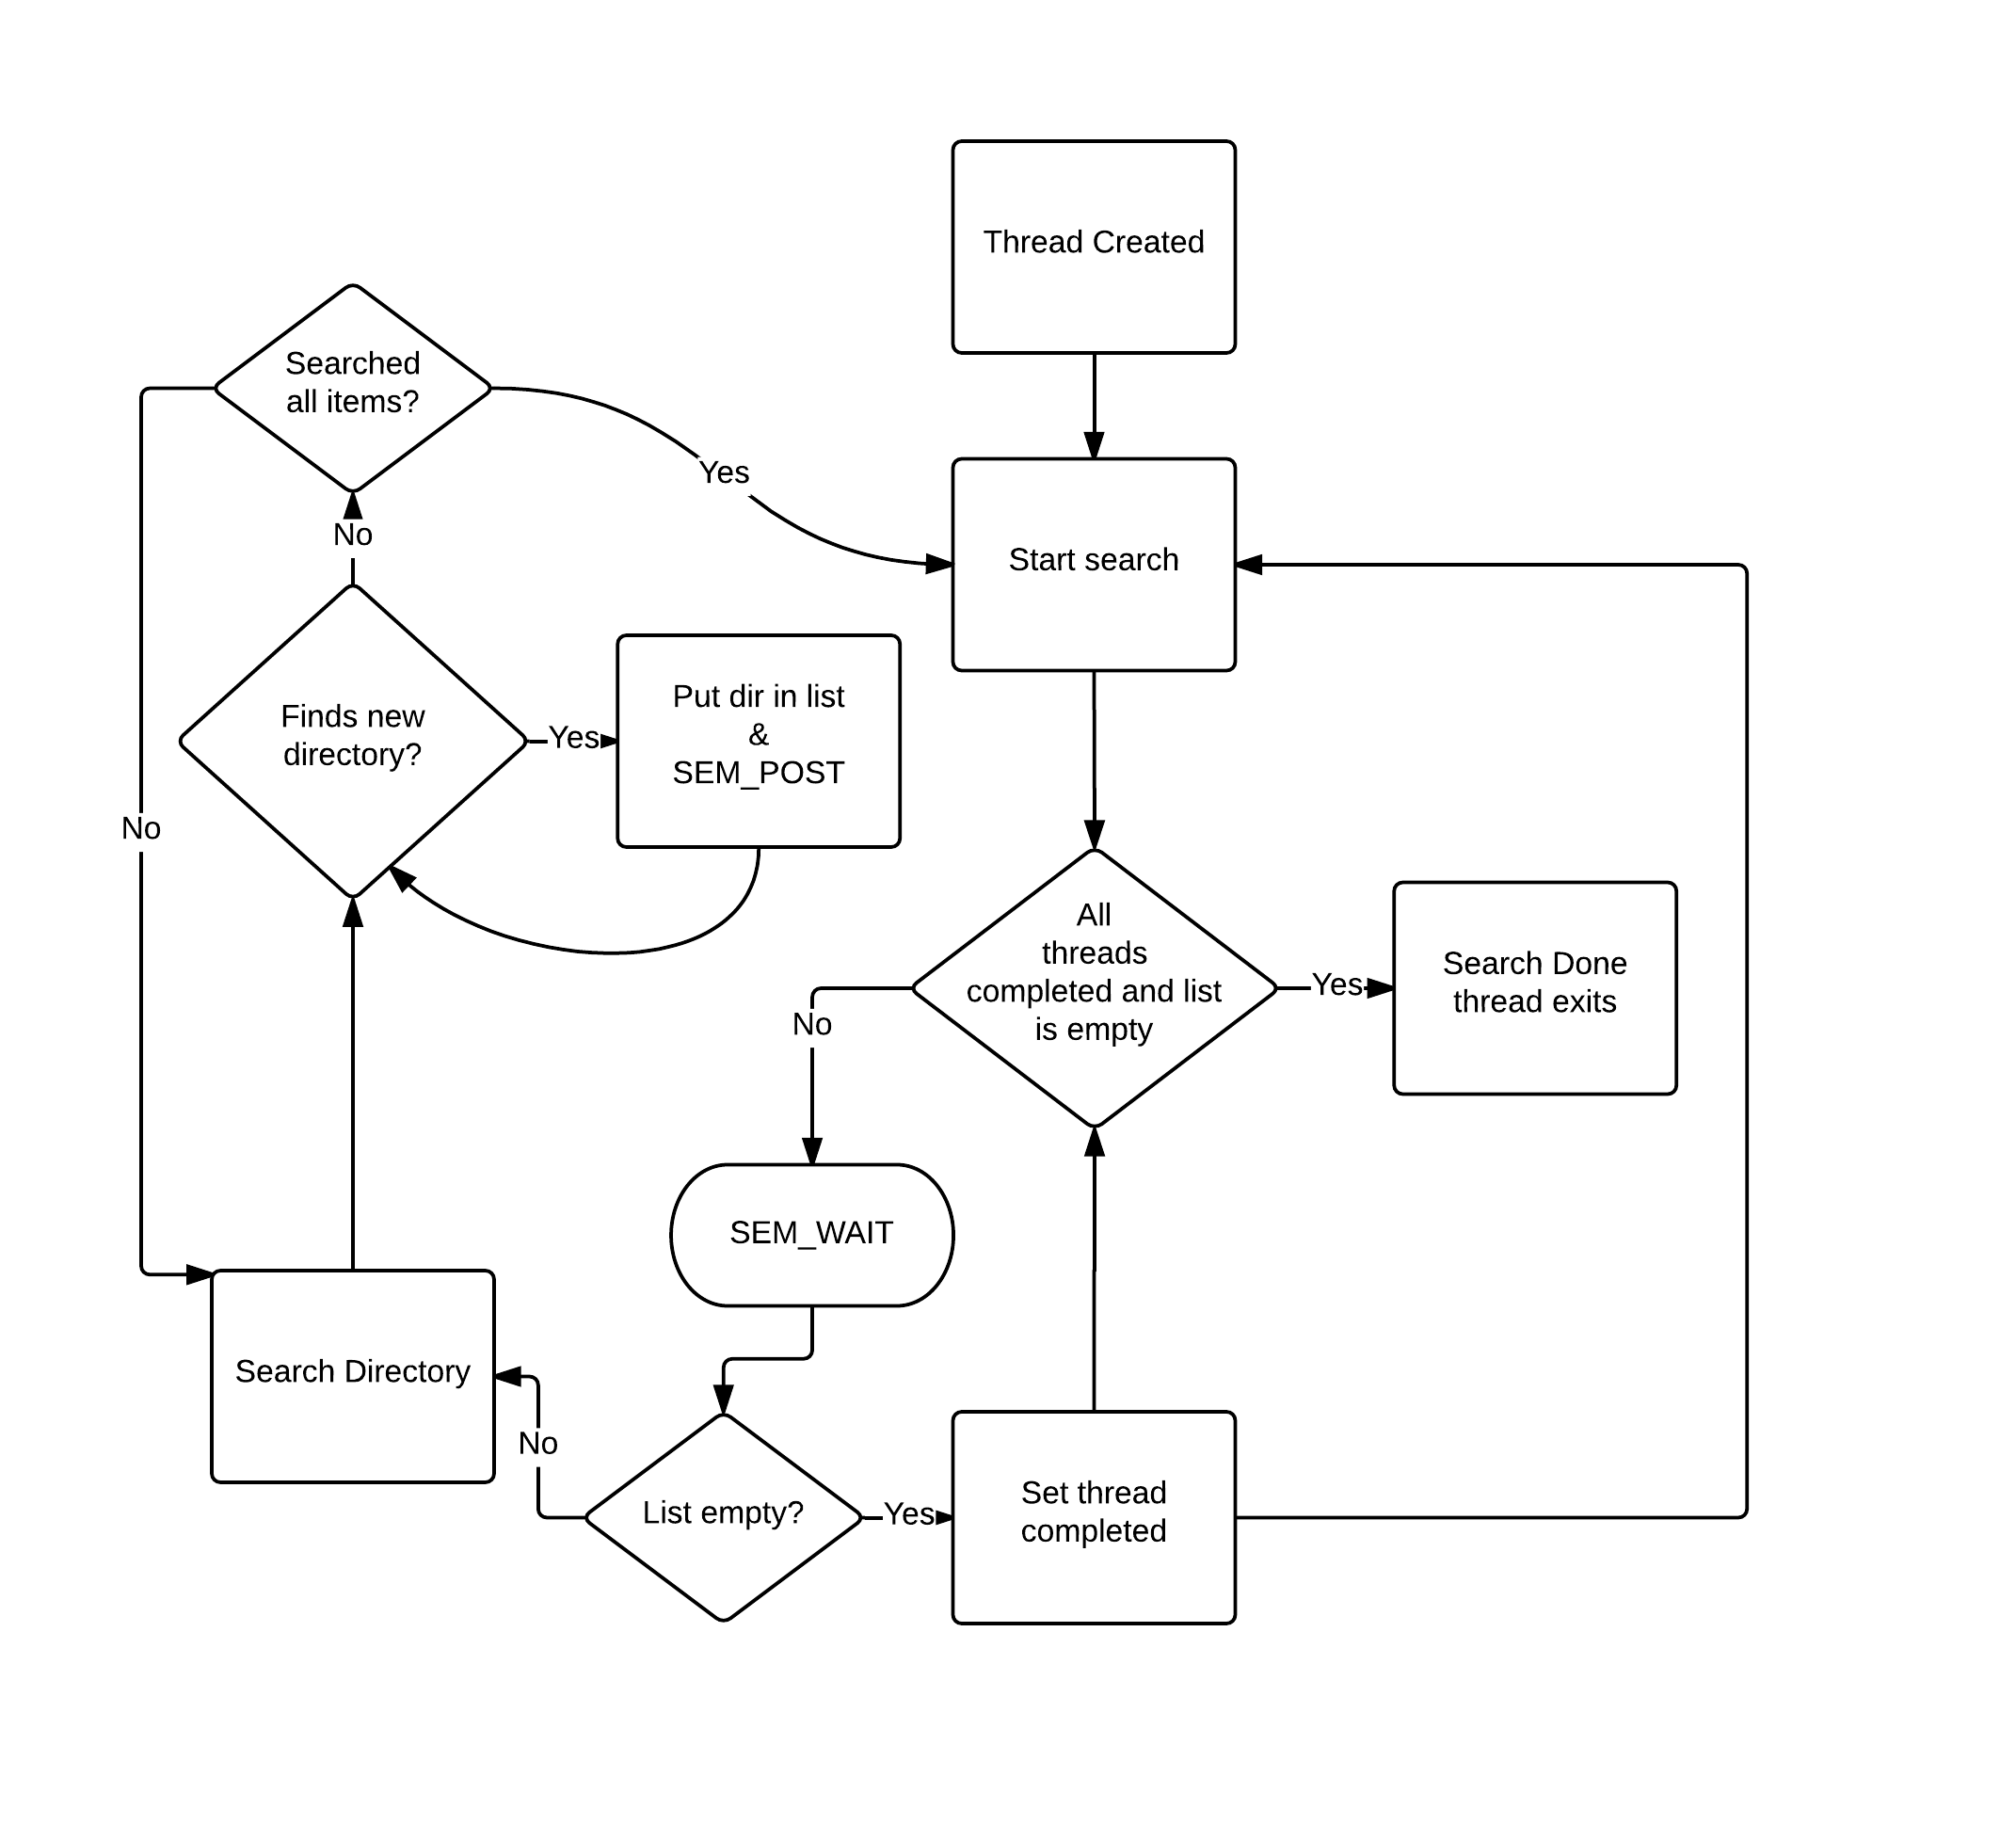
\includegraphics[width=1\textwidth]{m_find}
		\caption{\emph{Diagram över sökningsalgoritm}}
		\label{fig:find}
		\end{figure} 
						
						
		\Subsection{Går det snabbare med fler trådar?}
		  För att undersöka hur exekveringstiden ändrades så använde jag mig av två givna filer där det var möjligt att hämta den exakta tiden.
		  Den kod som borde vara del i tidtagningen är både skapandet av trådarna och startandet av dem.
		  
		  Jag körde tester där jag sökte igenom en mapp hierarki både med 1 tråd, 10 trådar, och 20 trådar. Hierarkierna jag testade mot var av olika storlek 
		  och jag testade även att söka efter olika filer som förekom olika ofta. Resultatet blev då som följer, där jag körde varje sökning tio gånger och tog medelvärdet av tiderna.
		
		  \begin{tabular}{| l | c | r | }
		  \hline
		  1 Tråd & 10 Trådar & 20 Trådar \\ \hline
		  1.88 & 1.8 & 1.9 \\ \hline
		  1.94 & 1.7 & 2.0 \\ \hline
		  4.0 & 8.0 & 9.6 \\ \hline
		  \end{tabular}
		  
		  Utifrån dessa tider för de olika metoderna och även en del odokumenterade tester så kommer jag till slutsatsen att sökningen oftast går lite snabbare med flera trådar
		  men om man söker igenom något litet så kommer det att kosta mera tid att skapa flera trådar än att låta en tråd göra jobbet. Trådar är kostsamt att skapa
		  och det tar tid, trådarna tävlar även om samma resurser så trådarna kommer att tävla emot varandra och detta medför att en tråd kan göra mera jobb än en annan.
		  Trådarna har även en del tid där de är oaktiva medans de väntar på att en annan tråd ska stoppa in jobb i kön, i fallet med en tråd så kommer den 
		  tråden alltid att jobba.
		  
		  En viss mängd trådar utför jobbet marginellt bättre än 1 eller 20 trådar, helt beroende från fall till fall.
		
		
		 \Subsection{Globala variabler}
		    Lösningen innehåller en del globala variabler, detta för att alla trådar ska kunna komma åt dem.
		    
		    \begin{itemize}
		     \item[dirList] Den länkade listan, alla trådar måste kunna hämta och lägga till sökvägar.
		     \item[nrOfThreads] En variabel som säger hur många trådar som ska köras, måste kunna nås av alla trådar för att dom ska kunna avgöra om dom är klara.
		     \item[threadsComplete] En global variabel som varje tråd ökar värdet med ett medans dom väntar och sänker värdet med ett om dom har arbete.
		     \item[fileToSearch] En variabel som innehåller namnet på den fil som ska sökas efter.
		     \item[lock] Ett mutex lås får att synkronisera användandet av vissa funktioner av trådarna.
		     \item[fileType] En variabel som berättar vilken sorts fil vi söker efter.
		     \item[semafor] En semafor som alla trådar använder sig av.
		     \item[threadSearchCount] En array som innehåller hur många sökvägar varje tråd har sökt igenom.
		    \end{itemize}

		\Section{Testkörningar}
		
		\subsection{Test 1}
		\begin{verbatim} 
itchy:~/edu/sysprog/lab5> ./mfind_p -p 3 /pkg/comsol comsol
/pkg/comsol/bin/comsol
/pkg/comsol/4.1/configuration/comsol
/pkg/comsol/4.1/bin/comsol
/pkg/comsol/4.1/bin/glnx86/comsol
/pkg/comsol/4.1/bin/glnxa64/comsol
/pkg/comsol/4.1/doc/html/comsol
/pkg/comsol/4.1/doc/pdf/comsol
Thread searched 87 directories
Thread searched 210 directories
Thread searched 92 directories
		 \end{verbatim}

		\subsection{Test 2}
		\begin{verbatim} 
itchy:~/edu/sysprog/lab5> ./mfind_p -p 3 /pkg/comsol/ /usr/local/bin/ comsol
/pkg/comsol//bin/comsol
/pkg/comsol//4.1/configuration/comsol
/pkg/comsol//4.1/bin/comsol
/usr/local/bin//comsol
/pkg/comsol//4.1/bin/glnx86/comsol
/pkg/comsol//4.1/bin/glnxa64/comsol
/pkg/comsol//4.1/doc/html/comsol
/pkg/comsol//4.1/doc/pdf/comsol
Thread searched 202 directories
Thread searched 104 directories
Thread searched 84 directories
		 \end{verbatim}
		 
		 
		\subsection{Test 3}
		\begin{verbatim} 
/pkg/comsol//4.1/configuration/comsol
/pkg/comsol//4.1/doc/html/comsol
/pkg/comsol//4.1/doc/pdf/comsol
Thread searched 84 directories
Thread searched 103 directories
Thread searched 203 directories
		 \end{verbatim}
		 
		\subsection{Test 4}
		\begin{verbatim} 
itchy:~/edu/sysprog/lab5> ./mfind_p -p 3 /opt/comsol/ /usr/local/bin/ comsol
cannot read dir /opt/comsol/: No such file or directory
Could not close file: Invalid argument
/usr/local/bin//comsol
Thread searched 1 directories
Thread searched 0 directories
Thread searched 0 directories
		 \end{verbatim}

		 \subsection{Test 5}
		\begin{verbatim} 
itchy:~/edu/sysprog/lab5> ./mfind_p -p 3 -t l /pkg/comsol/ /usr/local/bin/ comsol
/usr/local/bin//comsol
Thread searched 154 directories
Thread searched 77 directories
Thread searched 159 directories
		 \end{verbatim}

		 \subsection{Test 6}
		\begin{verbatim} 
itchy:~/edu/sysprog/lab5> ./mfind_p -p 3  ~mr/src cdecl.c
cannot read dir /Home/staff/mr/src: Permission denied
Could not close file: Invalid argument
Thread searched 0 directories
Thread searched 0 directories
Thread searched 0 directories
		 \end{verbatim}
		 
	\Section{Lösningens begränsningar}
		\emph{I detta avsnitt beskrivs alla begränsningar som lösningen av
			uppgiften innehåller. Detta innefattar även funna begränsningar
			som strider mot specifikationen.}
			
	\begin{enumerate}
	 \item I denna lösning så börjar trådarna arbeta direkt när dom skapas, detta medför att main tråden blir den sista att börja arbeta eftersom att den
	är upptagen med att skapa trådar. I vissa fall beroende på om antalet trådar som ska skapas och/eller katalogstrukturen som ska sökas igenom är för liten så kommer
	de första trådarna att hinna söka klart och därmed så resterande trådar inte söka igenom något och skapades i onödan.
	Det man kan göra för att motverka detta är att låta huvudtråden skapa alla trådar och sedan starta sökningen med alla trådar samtidigt.
	
	\item Operativsystemet har oftast en gräns på hur många trådar som får skapas, jag har satt en gräns på max 10000 trådar, för att det är inte resonabelt att använda så många trådar för denna uppgift.
	\end{enumerate}
 	
 	\Section{Reflektion och Diskussion}
 	Intressant att få prova på trådar i C miljö, har tidigare jobbat med trådar i Java och det var lite klurigare att arbeta med trådar i C till en början.
 	Det känndes svårt att göra en avvögning över hur man skulle göra med skapandet av trådar, när jag har provat med min lösning och gjort 30000 trådar och gjort sökningen ifrån \textbf{/} 
 	på min dator så har hälften av trådarna inte fått göra något arbete för att de trådar som skapats i början har redan hunnit söka klart. Och alternativet till detta skulle då vara att skapa 
 	alla trådar innan man påbörjar sökningen men det skulle inte vara effektivt om man skapade 300000 trådar och sedan ska börja sökningen på given sökväg och så är det bara en fil däri.
 	Samtidigt så i min implementation så i fallet att sökningen ska göras på en mapp som innehåller en fil så skapas 300000 trådar trots att det bara var en enda fil som skulle kollas.
 	
	
\end{document}